\documentclass[a4paper,12pt]{article}
\usepackage{graphicx}
\usepackage[dvipsnames]{xcolor}
\usepackage{wrapfig}
\usepackage{color}
\usepackage{graphicx}
\usepackage{subfigure}
\usepackage{multirow}
\usepackage[section] {placeins}
\usepackage{tikz}
\usepackage{amsmath}
\usetikzlibrary{matrix,calc}
\usetikzlibrary{positioning}
\usetikzlibrary{matrix}
\pgfdeclarelayer{background}
\pgfsetlayers{background,main}
\usepackage[hidelinks]{hyperref}

\definecolor{darkred}{rgb}{0,0,0.5}
\definecolor{darkgreen}{rgb}{0,0.5,0}
\definecolor{darkblue}{rgb}{0.5,0,0}
\hypersetup{ colorlinks, linkcolor=darkblue, filecolor=darkgreen, urlcolor=darkred, citecolor=darkblue}

\begin{document}
\begin{titlepage}
\begin{center}
	\textsc{\LARGE Indian Institute of Technology
			\\Bombay} \\[2.5cm]
	\begin{figure}[ht!]
	\begin{center}
		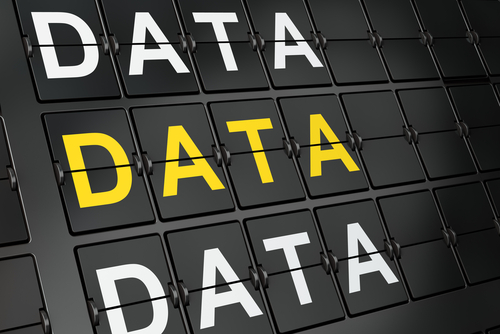
\includegraphics[scale = 1.4]{images/1}
	\end{center}
	\end{figure}

    \vspace*{-0.6cm}
	\hrule \hrule \hrule
	\vspace{0.5cm}	
	\textsc{\Large CS 492 : BTP Stage I}\\[0.5cm]
	% Title
	{\huge \bfseries Erlang Distributed File System (eDFS)} \\[0.5cm]
	\hrule \hrule \hrule
	\vspace{4cm}
	
	% Author and supervisor
	\begin{minipage}{0.4\textwidth}
	\begin{flushleft} \large
		\emph{By:} \\
		Aman Mangal (100050015)
	\end{flushleft}
	\end{minipage}
	\begin{minipage}{0.4\textwidth}
	\begin{flushright} \large
		\emph{Coordinator:} \\
		Prof. G. Sivakumar
	\end{flushright}
	\end{minipage}
	\vspace{0.5cm}
	
	% Bottom of the page
	{\large \today}
\end{center}
\end{titlepage}
\tableofcontents
\vspace{0.5cm}
\hrule \hrule \hrule
\newpage

\section{Introduction}
Distributed File System is an extension of File System which manages files and data on multiple storage devices and provides more performance and reliability using various modern techniques. Outside world only sees it as a single storage device and thus simplifying the interface to a great extent. It also provides location transparency and redundancy to improve data availability in case of failure or heavy load.

The idea of eDFS is to use Erlang distributive capabilities and build a fault tolerant, highly scalable and reliable distributed file system. We keep in mind the following assumption just like Google File System (GFS) \cite{ghemawat03} -
\begin{enumerate}
\item Component failures are norm rather than exception.
\item Files are huge by traditional standards.
\item Most files are mutated by appending rather than overwriting existing data, we may support concurrent append in future
\item Sequential access are more compared to random access. We optimize the file system for stream access.
\end{enumerate}

We optimize the file system for above cases. We may as well support other features in future. The performance is preferred over security. In the end of the project, we will also try to provide a Graphical User Interface which enables user and administrator to view the state of the machine.

\section{Design Overview}
\subsection{Architecture}
\subsection{Master Node (Metadata Server)}
\subsection{Metadata}
\subsection{Worker Node}

\section{System Interaction}
\subsection{Data Flow}
\subsection{Data Replication}
\subsection{Garbage Collection}

\section{Additional Features}

\section{Graphical User Interface}

\section{Testing}
\subsection{Map Reduce}

\begin{thebibliography}{9}
\bibitem{ghemawat03}
  \textsc{Sanjay Ghemawat, Howard Gobioff and Shun-Tak Leung}.
  The Google file system.
  \emph{In SOSP '03: Proceedings of the nineteenth ACM symposium on Operating systems principles}
  New York, NY, USA, 2003
\end{thebibliography}

\end{document}
